%=================================================================
% CSE 4345 — Big Data Analytics
% Week 8, Part 2: Seminal Research & Case Study
% Department of CSE, Premier University
%
% SEMINAL PAPER:
%   Kreps, Narkhede & Rao (2011) — Kafka: A Distributed Messaging
%   System for Log Processing. NetDB @ VLDB 2011. (cited >3,500)
%
% CASE STUDY:
%   Netflix Data Pipeline (2015–2021) — Kafka + Lambda/Kappa
%   architecture serving 200M subscribers at 100B events/day
%=================================================================

\documentclass[aspectratio=169,10pt]{beamer}

%---------- Packages ----------
\usepackage[utf8]{inputenc}
\usepackage[T1]{fontenc}
\usepackage{booktabs}
\usepackage{xcolor}
\usepackage{tikz}
\usetikzlibrary{shapes.geometric, positioning, arrows.meta,
                decorations.pathreplacing, patterns}
\usepackage{amsmath}
\usepackage{graphicx}
\usepackage{multicol}
\usepackage{enumerate}
\usepackage{array}

%---------- Theme ----------
\usetheme{Madrid}

%---------- Premier University Color Identity ----------
\definecolor{PUNavy}{RGB}{10,36,99}
\definecolor{PUGold}{RGB}{197,151,37}
\definecolor{PULightBlue}{RGB}{210,228,255}
\definecolor{PUTeal}{RGB}{0,100,100}
\definecolor{PUGray}{RGB}{90,90,90}
\definecolor{PURed}{RGB}{160,30,30}
\definecolor{PUGreen}{RGB}{30,120,60}
\definecolor{PUPurple}{RGB}{90,30,120}
\definecolor{PUOrange}{RGB}{190,90,20}

\setbeamercolor{palette primary}{bg=PUNavy, fg=white}
\setbeamercolor{palette secondary}{bg=PUNavy!85, fg=white}
\setbeamercolor{palette tertiary}{bg=PUNavy!70, fg=white}
\setbeamercolor{palette quaternary}{bg=PUNavy, fg=white}
\setbeamercolor{structure}{fg=PUNavy}
\setbeamercolor{title}{bg=PUNavy, fg=PUGold}
\setbeamercolor{subtitle}{fg=white}
\setbeamercolor{frametitle}{bg=PUNavy, fg=PUGold}
\setbeamercolor{alerted text}{fg=PUGold!85!black}
\setbeamercolor{block title}{bg=PUNavy, fg=white}
\setbeamercolor{block body}{bg=PULightBlue!45}
\setbeamercolor{block title alerted}{bg=PUGold!80!black, fg=white}
\setbeamercolor{block body alerted}{bg=PUGold!12}
\setbeamercolor{block title example}{bg=PUTeal, fg=white}
\setbeamercolor{block body example}{bg=PUTeal!10}
\setbeamercolor{section in toc}{fg=PUNavy}
\setbeamercolor{itemize item}{fg=PUGold!80!black}
\setbeamercolor{itemize subitem}{fg=PUNavy!70}

\setbeamertemplate{navigation symbols}{}
\setbeamertemplate{itemize item}{\scriptsize\raise1.5pt\hbox{\textbullet}}
\setbeamertemplate{itemize subitem}{\scriptsize\raise1pt\hbox{--}}

%---------- Section separator ----------
\AtBeginSection[]{
  \begin{frame}[plain]
    \vfill
    \centering
    \begin{beamercolorbox}[sep=12pt,center,shadow=true,rounded=true]{block title}
      \usebeamerfont{title}\insertsectionhead\par
    \end{beamercolorbox}
    \vfill
  \end{frame}
}

%---------- Helper: citation box ----------
\newenvironment{paperbox}[1]{%
  \setbeamercolor{block title}{bg=PUNavy!90,fg=PUGold}
  \setbeamercolor{block body}{bg=PUNavy!6}
  \begin{block}{#1}}{%
  \end{block}}

%---------- Custom footline ----------
\setbeamertemplate{footline}{
  \leavevmode\hbox{%
    \begin{beamercolorbox}[wd=.333\paperwidth,ht=2.25ex,dp=1ex,center]{palette primary}
      \usebeamerfont{author in head/foot}\insertshortauthor
    \end{beamercolorbox}%
    \begin{beamercolorbox}[wd=.334\paperwidth,ht=2.25ex,dp=1ex,center]{palette secondary}
      \usebeamerfont{title in head/foot}\insertshorttitle
    \end{beamercolorbox}%
    \begin{beamercolorbox}[wd=.333\paperwidth,ht=2.25ex,dp=1ex,right]{palette primary}
      \usebeamerfont{date in head/foot}
      \insertframenumber{} / \inserttotalframenumber\hspace*{2ex}
    \end{beamercolorbox}}%
  \vskip0pt%
}

%---------- Title metadata ----------
\title[CSE 4345 \textbar{} Week 8, Part 2]{CSE 4345: Big Data Analytics}
\subtitle{Week 8, Part 2 \textemdash\ Seminal Research \& Case Study}
\author[Dept.\ of CSE]{Department of Computer Science \& Engineering\\[4pt]
       \small Premier University, Chittagong}
\institute{}
\date{Semester 2026}

%=================================================================
\begin{document}
%=================================================================

%----------------------------------------------------------------
% TITLE SLIDE
%----------------------------------------------------------------
\begin{frame}
  \titlepage
\end{frame}

%----------------------------------------------------------------
% PART 2 OVERVIEW
%----------------------------------------------------------------
\begin{frame}{Part 2 Overview — Week 8}
  \begin{columns}[T]
    \column{0.47\textwidth}
      \begin{block}{Today's Agenda}
        \tableofcontents
      \end{block}

    \column{0.50\textwidth}
      \begin{exampleblock}{Seminal Paper Covered}
        \begin{enumerate}
          \item Kreps, J., Narkhede, N., \& Rao, J. (2011).
                \textit{Kafka: A Distributed Messaging System
                for Log Processing.}
                NetDB Workshop at VLDB 2011.
                Seattle, WA.
        \end{enumerate}
      \end{exampleblock}
      \vspace{6pt}
      \begin{alertblock}{Case Study}
        Netflix Data Pipeline (2015--2021):
        Kafka-backed Lambda/Kappa architecture serving
        \textbf{200M subscribers}, processing
        \textbf{100 billion events per day} for real-time
        personalisation and A/B testing.
      \end{alertblock}
      \vspace{4pt}
      \begin{block}{CLO Addressed}
        \textbf{CLO3, CLO4} — Explain distributed messaging;
        design stream-processing architectures\\
        \textbf{PLO(b,c)}
      \end{block}
  \end{columns}
\end{frame}

%================================================================
\section{Research Paper — Kreps, Narkhede \& Rao (2011): Kafka}
%================================================================

%----------------------------------------------------------------
\begin{frame}{Research Landscape: Distributed Messaging Timeline}
  \begin{center}
  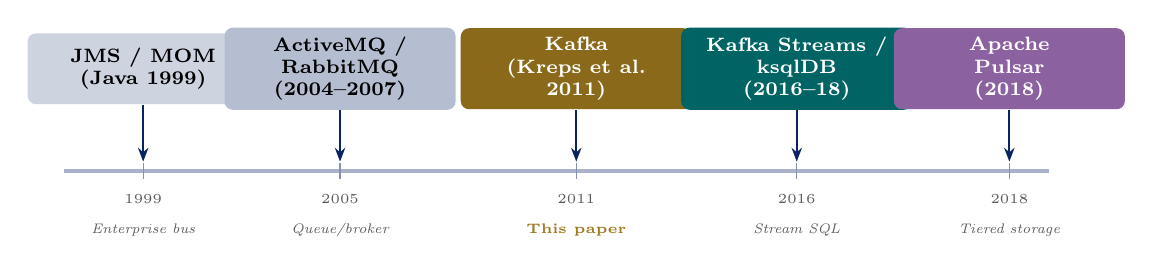
\begin{tikzpicture}[
      nbox/.style={rectangle, rounded corners=3pt, minimum width=2.9cm,
                   minimum height=0.9cm, text width=2.7cm, align=center,
                   font=\scriptsize\bfseries},
      arr/.style={-{Stealth[length=5pt]}, draw=PUNavy, thick}
    ]
    \draw[PUNavy!35, very thick] (0,0) -- (12.5,0);

    \node[nbox, fill=PUNavy!20]              (jms)  at (1.0, 1.3)
          {JMS / MOM\\(Java 1999)};
    \node[nbox, fill=PUNavy!30]              (amq)  at (3.5, 1.3)
          {ActiveMQ /\\RabbitMQ\\(2004--2007)};
    \node[nbox, fill=PUGold!70!black, text=white] (kaf) at (6.5, 1.3)
          {Kafka\\(Kreps et al.\\2011)};
    \node[nbox, fill=PUTeal, text=white]     (kst)  at (9.3, 1.3)
          {Kafka Streams /\\ksqlDB\\(2016--18)};
    \node[nbox, fill=PUPurple!70, text=white](pul)  at (12.0,1.3)
          {Apache\\Pulsar\\(2018)};

    \foreach \x/\y in {1.0/1999, 3.5/2005, 6.5/2011, 9.3/2016, 12.0/2018}{
      \draw[PUNavy!50] (\x,0.1) -- (\x,-0.1);
      \node[font=\tiny, text=PUGray] at (\x,-0.35) {\y};
    }

    \draw[arr] (jms)  -- (1.0,  0.12);
    \draw[arr] (amq)  -- (3.5,  0.12);
    \draw[arr] (kaf)  -- (6.5,  0.12);
    \draw[arr] (kst)  -- (9.3,  0.12);
    \draw[arr] (pul)  -- (12.0, 0.12);

    \node[font=\tiny\itshape, text=PUGray]           at (1.0,  -0.75) {Enterprise bus};
    \node[font=\tiny\itshape, text=PUGray]           at (3.5,  -0.75) {Queue/broker};
    \node[font=\tiny\bfseries, text=PUGold!80!black] at (6.5,  -0.75) {This paper};
    \node[font=\tiny\itshape, text=PUGray]           at (9.3,  -0.75) {Stream SQL};
    \node[font=\tiny\itshape, text=PUGray]           at (12.0, -0.75) {Tiered storage};
  \end{tikzpicture}
  \end{center}
  \vspace{4pt}
  \begin{alertblock}{Why Existing Systems Failed at LinkedIn's Scale}
    By 2010 LinkedIn was generating \textbf{billions of activity events per day}
    (profile views, connection clicks, job searches).
    ActiveMQ and RabbitMQ were designed for \emph{transactional messaging}
    (few thousand messages/sec, guaranteed delivery, complex routing).
    LinkedIn needed \textbf{sustained 100 MB/s throughput per broker},
    multi-day retention, and replay — none of which traditional MOM systems provided.
  \end{alertblock}
\end{frame}

%----------------------------------------------------------------
\begin{frame}{Kreps et al.\ (2011): Publication Context}
  \begin{columns}[T]
    \column{0.53\textwidth}
      \begin{paperbox}{Full Citation}
        Kreps, J., Narkhede, N., \& Rao, J. (2011).
        \textbf{Kafka: A Distributed Messaging System for Log Processing.}
        In \textit{Proceedings of the NetDB Workshop at the 37th
        International Conference on Very Large Data Bases (VLDB)}.
        Seattle, WA, USA.\\[5pt]
        \textbf{Venue:} NetDB Workshop at VLDB — focused workshop on
        networked and data-centre databases\\
        \textbf{Cited by:} $>$3{,}500 (Google Scholar, 2024)\\
        \textbf{Authors:} Jay Kreps (principal engineer), Neha Narkhede,
        Jun Rao — LinkedIn Data Infrastructure team
      \end{paperbox}
      \vspace{5pt}
      \begin{exampleblock}{The LinkedIn Origin Story}
        LinkedIn needed to collect activity data for its
        \textbf{People You May Know} and \textbf{Skills Endorsements}
        features.  The data collection system used a custom pipeline
        of Hadoop log files copied over NFS — fragile, high-latency,
        and impossible to replay.  Kafka was built to replace it
        and was open-sourced to Apache in 2012.
      \end{exampleblock}

    \column{0.44\textwidth}
      \begin{block}{The Core Abstraction}
        \begin{center}
        \large\color{PUNavy}
        \textit{``Kafka is a distributed,\\
        partitioned, replicated\\
        commit log service.''}
        \end{center}
        \vspace{4pt}
        \scriptsize
        Every message is appended to an \textbf{ordered, immutable log}
        per topic-partition.  Consumers read by advancing an
        \textbf{offset} — a simple integer pointer into the log.
        The broker never tracks what a consumer has read;
        the consumer does.  Replaying a stream means resetting
        the offset to any past position.
      \end{block}
  \end{columns}
\end{frame}

%----------------------------------------------------------------
\begin{frame}{Technical Contribution 1 — Topics, Partitions, Consumer Groups}
  \begin{columns}[T]
    \column{0.46\textwidth}
      \begin{block}{The Kafka Data Model}
        \begin{itemize}
          \item \textbf{Topic}: a named, ordered log — analogous to
                a database table but append-only
          \item \textbf{Partition}: a topic is split into $P$ partitions;
                each partition is an independent ordered log on one broker.
                Partitions enable \textbf{parallelism} and
                \textbf{horizontal scale}
          \item \textbf{Offset}: each message within a partition has a
                unique monotonically increasing integer offset.
                The consumer tracks its \emph{own} offset
                (stored in \texttt{\_\_consumer\_offsets} topic, Kafka 0.9+)
          \item \textbf{Consumer Group}: a set of consumers that
                together consume all partitions of a topic.
                Each partition is consumed by \textbf{exactly one}
                consumer in the group at a time — enabling
                ordered parallel processing
        \end{itemize}
      \end{block}

    \column{0.51\textwidth}
      \begin{center}
      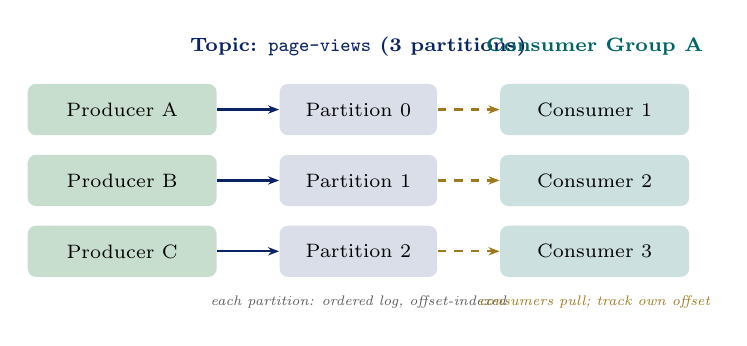
\begin{tikzpicture}[
          kbx/.style={rectangle, rounded corners=3pt, minimum width=2.4cm,
                      minimum height=0.65cm, align=center, font=\scriptsize},
          arr/.style={-{Stealth[length=4pt]}, draw=PUNavy, thick},
          darr/.style={-{Stealth[length=4pt]}, draw=PUGold!80!black,
                       thick, dashed}
        ]
        % Producers
        \node[kbx, fill=PUGreen!25] (pa) at (-3.0, 3.2) {Producer A};
        \node[kbx, fill=PUGreen!25] (pb) at (-3.0, 2.3) {Producer B};
        \node[kbx, fill=PUGreen!25] (pc) at (-3.0, 1.4) {Producer C};

        % Topic partitions (broker)
        \node[font=\scriptsize\bfseries, text=PUNavy] at (0, 4.0)
              {Topic: \texttt{page-views} (3 partitions)};
        \node[kbx, fill=PUNavy!15, minimum width=2.0cm]
              (p0) at (0, 3.2) {Partition 0};
        \node[kbx, fill=PUNavy!15, minimum width=2.0cm]
              (p1) at (0, 2.3) {Partition 1};
        \node[kbx, fill=PUNavy!15, minimum width=2.0cm]
              (p2) at (0, 1.4) {Partition 2};

        % Consumer group
        \node[font=\scriptsize\bfseries, text=PUTeal] at (3.0, 4.0)
              {Consumer Group A};
        \node[kbx, fill=PUTeal!20] (ca) at (3.0, 3.2) {Consumer 1};
        \node[kbx, fill=PUTeal!20] (cb) at (3.0, 2.3) {Consumer 2};
        \node[kbx, fill=PUTeal!20] (cc) at (3.0, 1.4) {Consumer 3};

        % Producer arrows (hash partitioning)
        \draw[arr] (pa) -- (p0);
        \draw[arr] (pb) -- (p1);
        \draw[arr] (pc) -- (p2);

        % Consumer pull arrows
        \draw[darr] (p0) -- (ca);
        \draw[darr] (p1) -- (cb);
        \draw[darr] (p2) -- (cc);

        % Offset annotation
        \node[font=\tiny\itshape, text=PUGray] at (0, 0.75)
              {each partition: ordered log, offset-indexed};
        \node[font=\tiny\itshape, text=PUGold!80!black] at (3.0, 0.75)
              {consumers pull; track own offset};
      \end{tikzpicture}
      \end{center}
  \end{columns}
\end{frame}

%----------------------------------------------------------------
\begin{frame}{Technical Contribution 2 — Log Storage \& Zero-Copy}
  \begin{columns}[T]
    \column{0.50\textwidth}
      \begin{block}{Partition as a Segmented Append-Only Log}
        Each partition is stored as a sequence of \textbf{segment files}
        on the broker's local disk:
        \begin{itemize}
          \item Each segment: one \texttt{.log} file (message data)
                + one \texttt{.index} file (offset $\to$ byte position)
          \item Active segment: the last segment, open for appends
          \item Old segments: closed, immutable; eligible for deletion
                after the \textbf{retention period} (default 7 days)
                or when total log size exceeds a threshold
          \item \textbf{Sequential writes only}: the OS page cache
                prefetches the next pages, achieving
                near-disk-bandwidth throughput without SSD
        \end{itemize}
      \end{block}
      \vspace{4pt}
      \begin{alertblock}{Zero-Copy Transfer (sendfile)}
        Traditional broker: disk $\to$ kernel buffer $\to$
        user space $\to$ socket buffer $\to$ NIC (\textbf{4 copies}).\\
        Kafka: disk $\to$ kernel buffer $\to$ NIC directly
        via Linux \texttt{sendfile()} syscall (\textbf{2 copies}).\\
        Result: \textbf{$2\times$ throughput, CPU near zero}.
      \end{alertblock}

    \column{0.47\textwidth}
      \begin{center}
      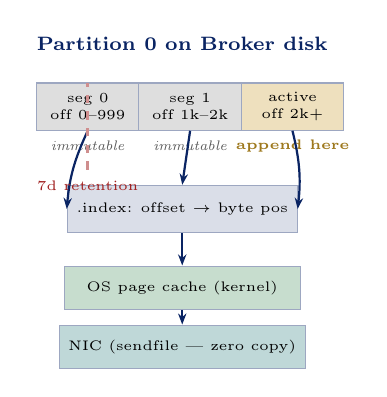
\begin{tikzpicture}[
          seg/.style={rectangle, minimum width=1.3cm, minimum height=0.6cm,
                      align=center, font=\tiny, draw=PUNavy!40},
          arr/.style={-{Stealth[length=4pt]}, draw=PUNavy, thick}
        ]
        % Log segments
        \node[font=\scriptsize\bfseries, text=PUNavy] at (1.5, 4.0)
              {Partition 0 on Broker disk};

        \node[seg, fill=PUGray!20]   (s0) at (0.3, 3.2)
              {seg 0\\off 0--999};
        \node[seg, fill=PUGray!20]   (s1) at (1.6, 3.2)
              {seg 1\\off 1k--2k};
        \node[seg, fill=PUGold!30]   (s2) at (2.9, 3.2)
              {active\\off 2k+};

        \node[font=\tiny\itshape, text=PUGray] at (0.3, 2.7)
              {immutable};
        \node[font=\tiny\itshape, text=PUGray] at (1.6, 2.7)
              {immutable};
        \node[font=\tiny\bfseries, text=PUGold!80!black] at (2.9, 2.7)
              {append here};

        % Offset index
        \node[seg, fill=PUNavy!15, minimum width=2.8cm]
              (idx) at (1.5, 1.9) {.index: offset $\to$ byte pos};

        \draw[arr] (s0.south) to[bend right=10] (idx.west);
        \draw[arr] (s1.south) -- (idx.north);
        \draw[arr] (s2.south) to[bend left=10]  (idx.east);

        % Retention
        \draw[PURed!50, very thick, dashed]
              (0.3, 2.4) -- (0.3, 3.5);
        \node[font=\tiny, text=PURed] at (0.3, 2.2)
              {7d retention};

        % sendfile path
        \node[seg, fill=PUGreen!25, minimum width=3.0cm,
              minimum height=0.55cm]
              (sf) at (1.5, 0.9) {OS page cache (kernel)};
        \node[seg, fill=PUTeal!25, minimum width=3.0cm,
              minimum height=0.55cm]
              (nic) at (1.5, 0.15) {NIC (sendfile — zero copy)};
        \draw[arr] (idx.south) -- (sf.north);
        \draw[arr] (sf.south)  -- (nic.north);
      \end{tikzpicture}
      \end{center}
  \end{columns}
\end{frame}

%----------------------------------------------------------------
\begin{frame}{Technical Contribution 3 — Performance Benchmarks}
  \begin{columns}[T]
    \column{0.52\textwidth}
      \begin{block}{Producer Throughput (from the paper)}
        Benchmark: single broker, 6$\times$ 7200~RPM SATA,
        10~GbE NIC, 100-byte messages, no replication.
        \begin{center}
        \renewcommand{\arraystretch}{1.3}
        \begin{tabular}{@{}lrr@{}}
          \toprule
          \textbf{System} & \textbf{MB/s} & \textbf{Msgs/sec} \\
          \midrule
          ActiveMQ        &  4.3 &   43{,}000 \\
          RabbitMQ        & 14.7 &  147{,}000 \\
          \textbf{Kafka}  & \textbf{50.5} & \textbf{505{,}000} \\
          \bottomrule
        \end{tabular}
        \end{center}
      \end{block}
      \vspace{5pt}
      \begin{block}{Consumer Throughput}
        \begin{center}
        \renewcommand{\arraystretch}{1.3}
        \begin{tabular}{@{}lrr@{}}
          \toprule
          \textbf{System} & \textbf{MB/s} & \textbf{Msgs/sec} \\
          \midrule
          ActiveMQ       &  4.0 &   40{,}000 \\
          RabbitMQ       &  8.2 &   82{,}000 \\
          \textbf{Kafka} & \textbf{22.0} & \textbf{220{,}000} \\
          \bottomrule
        \end{tabular}
        \end{center}
      \end{block}

    \column{0.45\textwidth}
      \begin{exampleblock}{Why Kafka is Faster: Summary}
        \begin{enumerate}
          \item \textbf{Sequential disk writes}: spinning disk
                sequential I/O ($\sim$600~MB/s) vs.\ random I/O
                ($\sim$100~MB/s) — $6\times$ advantage
          \item \textbf{Zero-copy}: \texttt{sendfile()} eliminates
                2 user-space copies and 2 context switches
          \item \textbf{Batch compression}: producer batches messages
                into a single compressed record set before sending;
                compression ratio 5--10$\times$ for log data
          \item \textbf{No per-message ACK}: broker ACKs a batch,
                not each message individually
          \item \textbf{Consumer pull}: broker never maintains
                per-consumer queues; a single log serves all consumers
        \end{enumerate}
      \end{exampleblock}
      \vspace{4pt}
      \begin{alertblock}{Kafka Today}
        Production Kafka clusters at LinkedIn (2021):
        \textbf{1.8 trillion messages/day}, 4{,}400 brokers,
        peak \textbf{13 million messages/sec}.
      \end{alertblock}
  \end{columns}
\end{frame}

%----------------------------------------------------------------
\begin{frame}{Impact Today — Kreps et al.\ (2011)}
  \begin{columns}[T]
    \column{0.50\textwidth}
      \begin{block}{Kafka's Lasting Influence}
        \begin{itemize}
          \item \textbf{Kafka Streams} (2016): lightweight stream
                processing library within Kafka — stateful
                transformations without Flink or Spark
          \item \textbf{ksqlDB} (2017): streaming SQL on Kafka topics;
                \texttt{CREATE STREAM AS SELECT} pushes continuous
                query results into a new topic
          \item \textbf{Kafka Connect} (2015): plug-in connectors for
                200+ source/sink systems (JDBC, S3, Elasticsearch);
                replaces Sqoop and Flume for most use cases
          \item \textbf{Schema Registry} (Confluent, 2015): Avro/Protobuf
                schema enforcement per topic; consumer can deserialise
                messages written by any past producer version
          \item \textbf{Exactly-once semantics} (Kafka 0.11, 2017):
                idempotent producer + transactional API; eliminates
                duplicates across produce + consume + produce pipelines
          \item \textbf{Tiered storage} (Kafka 3.6, 2023):
                offload old segments to S3; cost reduction for
                long-retention topics
        \end{itemize}
      \end{block}

    \column{0.47\textwidth}
      \begin{exampleblock}{Harvard CS265 / CMU 15-721 Perspective}
        \begin{itemize}
          \item Harvard CS265 presents Kafka's partition-offset model
                as an instance of \textbf{total order broadcast} —
                equivalent to Paxos log replication but implemented
                with leader-based ISR (In-Sync Replicas)
          \item CMU 15-721 uses Kafka as the canonical example of a
                \textbf{log-structured storage engine}:
                the partition log is exactly a single-writer LSM-tree
                without compaction — because messages are never updated
          \item Both courses note that Kafka's \textbf{consumer group
                rebalancing} (partition reassignment on join/leave)
                is a distributed systems challenge equivalent to
                consistent hashing with virtual nodes
        \end{itemize}
      \end{exampleblock}
      \vspace{4pt}
      \begin{alertblock}{CLO3/CLO4 Connection}
        Kafka directly addresses CLO3 (explaining distributed messaging)
        and CLO4 (designing event-driven pipelines for real-world scale).
      \end{alertblock}
  \end{columns}
\end{frame}

%================================================================
\section{Case Study — Netflix Data Pipeline (2015--2021)}
%================================================================

%----------------------------------------------------------------
\begin{frame}{Netflix's Event-Driven Scale}
  \begin{columns}[T]
    \column{0.52\textwidth}
      \begin{block}{Why Netflix Needed an Industrial-Scale Pipeline}
        Netflix (200M subscribers, 2021) generates:
        \begin{itemize}
          \item \textbf{Playback events}: play, pause, seek, buffering,
                quality switch — for every stream on every device
          \item \textbf{UI interactions}: hover, click, scroll on the
                home screen catalogue — drives A/B testing
          \item \textbf{Search queries}: what users search, what they
                select from results
          \item \textbf{Error events}: client-side errors, CDN cache
                misses, codec failures — for reliability monitoring
          \item \textbf{Scale}: $\approx$\textbf{100 billion events/day},
                peaking at \textbf{1.3 million events/second}
                during prime-time (Fri 9~pm US Eastern)
        \end{itemize}
        All events flow through \textbf{Kafka} before being processed
        by two parallel pipelines: real-time (speed) and batch.
      \end{block}

    \column{0.45\textwidth}
      \begin{alertblock}{What Fails Without This Pipeline}
        \begin{itemize}
          \item \textbf{Personalisation lag}: if the home screen
                re-ranks titles only once per day, a user who just
                finished \textit{Stranger Things S4} still sees S3 at
                the top the next morning
          \item \textbf{A/B testing blindness}: Netflix runs
                $>$200 concurrent A/B tests; without real-time event
                ingestion, test results take days instead of hours
          \item \textbf{Reliability gaps}: stream rebuffering events
                alert the CDN team; without real-time stream processing,
                a region-wide outage takes 30 minutes to detect
        \end{itemize}
      \end{alertblock}
  \end{columns}
\end{frame}

%----------------------------------------------------------------
\begin{frame}{Netflix Lambda + Kappa Architecture}
  \begin{columns}[T]
    \column{0.48\textwidth}
      \begin{block}{Lambda Architecture at Netflix}
        \textbf{Speed layer} (latency $<$1 minute):
        \begin{itemize}
          \item Kafka $\to$ \textbf{Flink} (event-time windowing)
          \item Outputs: real-time dashboards (Kibana),
                alert triggers, live A/B test counters
        \end{itemize}
        \vspace{4pt}
        \textbf{Batch layer} (latency $\sim$1 day):
        \begin{itemize}
          \item Kafka $\to$ S3 (via Kafka S3 sink connector)
          \item S3 $\to$ \textbf{Spark + Apache Iceberg}
                (hourly/daily ETL jobs on EMR)
          \item Outputs: ML training datasets, billing aggregates,
                long-term analytics warehouse
        \end{itemize}
        \vspace{4pt}
        \textbf{Serving layer}:
        \begin{itemize}
          \item \textbf{Cassandra}: low-latency user-state reads
                (last watched, continue-watching row)
          \item \textbf{Druid}: interactive OLAP on event aggregates
                for product and data science teams
        \end{itemize}
      \end{block}

    \column{0.49\textwidth}
      \begin{center}
      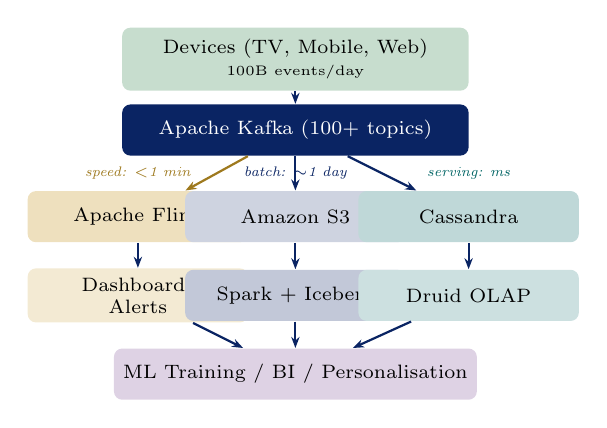
\begin{tikzpicture}[
          nb/.style={rectangle, rounded corners=3pt, minimum width=2.8cm,
                     minimum height=0.65cm, align=center, font=\scriptsize},
          arr/.style={-{Stealth[length=4pt]}, draw=PUNavy, thick},
          sarr/.style={-{Stealth[length=4pt]}, draw=PUGold!80!black,
                       thick}
        ]
        % Sources
        \node[nb, fill=PUGreen!25, minimum width=4.4cm,
              minimum height=0.8cm]
              (src) at (0, 4.5)
              {Devices (TV, Mobile, Web)\\{\tiny 100B events/day}};

        % Kafka
        \node[nb, fill=PUNavy, text=white, minimum width=4.4cm]
              (kaf) at (0, 3.6) {Apache Kafka (100+ topics)};

        % Speed layer
        \node[nb, fill=PUGold!30] (flink)  at (-2.0, 2.5) {Apache Flink};
        \node[nb, fill=PUGold!20] (dash)   at (-2.0, 1.5) {Dashboards\\Alerts};

        % Batch layer
        \node[nb, fill=PUNavy!20] (s3)     at (0,    2.5) {Amazon S3};
        \node[nb, fill=PUNavy!25] (spark)  at (0,    1.5) {Spark + Iceberg};

        % Serving layer
        \node[nb, fill=PUTeal!25] (cass)   at (2.2,  2.5) {Cassandra};
        \node[nb, fill=PUTeal!20] (druid)  at (2.2,  1.5) {Druid OLAP};

        % Output
        \node[nb, fill=PUPurple!20, minimum width=4.4cm]
              (out) at (0, 0.5) {ML Training / BI / Personalisation};

        \draw[arr] (src)   -- (kaf);
        \draw[sarr](kaf)   -- (flink);
        \draw[arr] (kaf)   -- (s3);
        \draw[arr] (kaf)   -- (cass);
        \draw[arr] (flink) -- (dash);
        \draw[arr] (s3)    -- (spark);
        \draw[arr] (cass)  -- (druid);
        \draw[arr] (dash)  -- (out);
        \draw[arr] (spark) -- (out);
        \draw[arr] (druid) -- (out);

        \node[font=\tiny\itshape, text=PUGold!80!black] at (-2.0, 3.05)
              {speed: $<$1 min};
        \node[font=\tiny\itshape, text=PUNavy]          at (0, 3.05)
              {batch: $\sim$1 day};
        \node[font=\tiny\itshape, text=PUTeal]          at (2.2, 3.05)
              {serving: ms};
      \end{tikzpicture}
      \end{center}
  \end{columns}
\end{frame}

%----------------------------------------------------------------
\begin{frame}{Netflix A/B Testing Pipeline on Kafka}
  \begin{columns}[T]
    \column{0.52\textwidth}
      \begin{block}{Why A/B Testing Requires Real-Time Events}
        Netflix runs $>$\textbf{200 simultaneous A/B tests}:
        different artwork thumbnails, autoplay delays,
        recommendation algorithms, UI layouts.
        Each test needs:
        \begin{enumerate}
          \item \textbf{Assignment}: user bucketed into control
                or treatment at login time (stored in Cassandra)
          \item \textbf{Exposure event}: logged to Kafka when the
                user sees the tested feature
          \item \textbf{Outcome events}: play, click, skip, subscribe
                — logged to Kafka within seconds of the action
          \item \textbf{Statistical aggregation}: Flink window joins
                assignment $\bowtie$ exposure $\bowtie$ outcome events
                to compute conversion rates \emph{in real time}
          \item \textbf{Result}: experiment dashboard updated every
                \textbf{5 minutes}; engineers ship winning variants
                the \emph{same day} instead of waiting for a batch run
        \end{enumerate}
      \end{block}

    \column{0.45\textwidth}
      \begin{block}{Scale Numbers (Netflix, 2021)}
        \renewcommand{\arraystretch}{1.25}
        \begin{tabular}{@{}ll@{}}
          \toprule
          \textbf{Metric}             & \textbf{Value} \\
          \midrule
          Subscribers                 & 200M \\
          Events per day              & 100 billion \\
          Peak events per second      & 1.3 million \\
          Kafka topics                & 4{,}000+ \\
          Kafka brokers               & 2{,}000+ \\
          Message retention           & 7 days \\
          Flink jobs (speed layer)    & 150+ \\
          Concurrent A/B tests        & $>$200 \\
          Experiment result latency   & 5 minutes \\
          S3 batch pipeline cadence   & Hourly \\
          Iceberg table count         & 5{,}000+ \\
          \bottomrule
        \end{tabular}
      \end{block}
      \vspace{4pt}
      \begin{exampleblock}{Netflix's Kafka Contribution}
        Netflix open-sourced \textbf{Metacat} (data catalog) and
        co-developed \textbf{Apache Iceberg} (table format for S3 ACID
        writes), both driven by their batch pipeline requirements.
      \end{exampleblock}
  \end{columns}
\end{frame}

%----------------------------------------------------------------
\begin{frame}{Lessons Learned \& Discussion Questions}
  \begin{columns}[T]
    \column{0.52\textwidth}
      \begin{block}{Key Lessons from Netflix's Pipeline}
        \begin{enumerate}
          \item \textbf{Kafka as the single source of truth}:
                all events written to Kafka first; the speed and
                batch layers are both consumers of the same topic —
                eliminating the data inconsistency problem of classic
                Lambda (two separate ingestion paths)
          \item \textbf{Retention enables reprocessing}:
                7-day retention lets Netflix replay any event window
                when a Flink job has a bug or a Spark job fails
          \item \textbf{Kappa simplification}: Netflix increasingly
                moved batch jobs to Flink stream processing
                (processing historical S3 data as a bounded stream),
                reducing pipeline complexity
          \item \textbf{Schema Registry is non-negotiable at scale}:
                4{,}000 topics $\times$ evolving schemas $\Rightarrow$
                consumer breakage without schema governance
          \item \textbf{Backpressure is the real production problem}:
                during Super Bowl commercials, event rates spike
                $5\times$; Kafka's durable log absorbs the burst;
                Flink consumers catch up within minutes
        \end{enumerate}
      \end{block}

    \column{0.45\textwidth}
      \begin{alertblock}{Discussion Questions \textmd{\tiny (CLO3, CLO4)}}
        \begin{enumerate}
          \item Netflix's Kafka cluster handles 1.3M events/sec at peak
                across 4{,}000 topics.
                If each topic has 12 partitions, calculate the
                \textbf{minimum number of brokers} needed assuming
                each broker handles 50{,}000 partitions and a
                replication factor of 3.
                \textit{[CLO4 — Apply]}
          \item A Flink job joins three Kafka streams:
                \texttt{assignments}, \texttt{exposures}, and
                \texttt{outcomes} on \texttt{user\_id}.
                Events may arrive out of order by up to 30 seconds.
                Design an \textbf{event-time window} strategy
                (window size, watermark lag, allowed lateness)
                and justify each choice.
                \textit{[CLO4 — Design]}
          \item Netflix uses both Lambda (speed + batch) and Kappa
                (stream-only) architectures for different pipelines.
                Identify \textbf{two workloads} where Lambda is
                preferable to Kappa and explain why stream reprocessing
                alone is insufficient.
                \textit{[CLO3 — Evaluate]}
        \end{enumerate}
      \end{alertblock}
  \end{columns}
\end{frame}

%================================================================
\section{Live Exercise}
%================================================================

%----------------------------------------------------------------
\begin{frame}[fragile]{Live Exercise — Kafka Producer/Consumer in Python}
  \begin{columns}[T]
    \column{0.50\textwidth}
      \begin{block}{Task (25 minutes, pairs)}
        Simulate a Kafka producer/consumer pipeline using the
        \textbf{kafka-python} library with a local single-broker
        cluster (Docker Compose provided below).\\[5pt]
        \textbf{Goals}:
        \begin{enumerate}\setlength\itemsep{1pt}
          \item Run the producer — send 1{,}000 synthetic
                Netflix play events to topic \texttt{play-events}.
          \item Run the consumer — read all messages,
                count plays per \texttt{content\_id}.
          \item Reset the consumer offset to the \emph{beginning}
                and re-consume — verify idempotent results.
          \item Change the consumer group ID and observe that
                a new group starts from offset 0.
        \end{enumerate}
      \end{block}
      \vspace{4pt}
      \begin{exampleblock}{Quick-start}
        \scriptsize\texttt{pip install kafka-python}\\
        \scriptsize\texttt{docker run -p 9092:9092 apache/kafka:3.7.0}
      \end{exampleblock}

    \column{0.47\textwidth}
      \begin{exampleblock}{Python Skeleton}
        \scriptsize
        \begin{verbatim}
import json, random, time
from kafka import KafkaProducer, KafkaConsumer

TOPIC   = "play-events"
BROKER  = "localhost:9092"
CONTENT = [f"show_{i}" for i in range(20)]

# --- Producer ---
producer = KafkaProducer(
  bootstrap_servers=BROKER,
  value_serializer=lambda v:
      json.dumps(v).encode())

for _ in range(1_000):
    event = {
      "user_id":    random.randint(1, 500),
      "content_id": random.choice(CONTENT),
      "action":     random.choice(
                      ["play","pause","seek"]),
      "ts":         int(time.time())
    }
    producer.send(TOPIC, event)
producer.flush()
print("Produced 1,000 events")

# --- Consumer ---
consumer = KafkaConsumer(
  TOPIC,
  bootstrap_servers=BROKER,
  group_id="cse4345-group",
  auto_offset_reset="earliest",
  value_deserializer=lambda m:
      json.loads(m.decode()))

counts = {}
for msg in consumer:
    cid = msg.value["content_id"]
    counts[cid] = counts.get(cid, 0) + 1
    if sum(counts.values()) >= 1_000:
        break
print(sorted(counts.items(),
             key=lambda x: -x[1])[:5])
        \end{verbatim}
      \end{exampleblock}
  \end{columns}
\end{frame}

%================================================================
\section*{References}
%================================================================

%----------------------------------------------------------------
\begin{frame}{References}
  \begin{block}{Seminal Paper}
    \begin{itemize}
      \item Kreps, J., Narkhede, N., \& Rao, J. (2011).
            Kafka: A distributed messaging system for log processing.
            \textit{Proc.\ NetDB Workshop at VLDB}.
    \end{itemize}
  \end{block}
  \vspace{4pt}
  \begin{block}{Textbooks \textmd{[SA], [TE], [TW]}}
    \begin{itemize}
      \item \textbf{[SA]} Acharya, S., \& Chellappan, S. (2015).
            \textit{Big Data and Analytics}
            (Ch.~8 — Real-Time Streaming). Wiley.
      \item \textbf{[TE]} Erl, T., Khattak, W., \& Buhler, P. (2016).
            \textit{Big Data Fundamentals}
            (Ch.~10 — Lambda and Kappa Architectures). Prentice Hall.
      \item \textbf{[TW]} White, T. (2015).
            \textit{Hadoop: The Definitive Guide}, 4th ed.
            (Ch.~14 — Flume; Ch.~15 -- Sqoop). O'Reilly.
    \end{itemize}
  \end{block}
  \vspace{4pt}
  \begin{block}{Case Study Sources}
    \begin{itemize}
      \item Arun, M. (2016).
            Kafka inside Keystone Pipeline.
            \textit{Netflix Tech Blog}.
      \item Goodhope, K., et al. (2012).
            Building LinkedIn's Real-time Activity Data Pipeline.
            \textit{IEEE Data Engineering Bulletin, 35}(2).
    \end{itemize}
  \end{block}
\end{frame}

%----------------------------------------------------------------
\begin{frame}{Closing — Week 8, Part 2}
  \begin{columns}[T]
    \column{0.52\textwidth}
      \begin{block}{Key Takeaways}
        \begin{itemize}
          \item Kafka's insight — \textbf{treat the log as the database}
                — turned a simple append-only file into the backbone
                of modern event-driven architecture
          \item \textbf{Zero-copy + sequential I/O} are the two
                engineering decisions that explain Kafka's $10\times$
                throughput advantage over traditional MOM systems;
                they are also why Kafka runs on spinning disk at
                near-SSD throughput
          \item Netflix's pipeline shows that \textbf{Kafka's retention
                collapses the Lambda architecture's complexity}: when
                speed and batch layers both read from the same durable
                log, the dual-ingestion problem disappears
          \item \textbf{Schema governance and exactly-once semantics}
                are the operational challenges that dominate after
                the initial Kafka deployment — not throughput
        \end{itemize}
      \end{block}

    \column{0.45\textwidth}
      \begin{alertblock}{Quote of the Week}
        \begin{center}
        \large\itshape
        ``A log is perhaps the simplest
        possible storage abstraction.
        It is an append-only, totally
        ordered sequence of records
        ordered by time.''
        \end{center}
        \begin{flushright}
        \small --- Jay Kreps, \textit{The Log} (2013)
        \end{flushright}
      \end{alertblock}
      \vspace{6pt}
      \begin{exampleblock}{Part 1 Preview — Week 9}
        \textbf{Visualisation Principles, D3, Tableau \& Grafana}\\[3pt]
        \begin{itemize}\setlength\itemsep{1pt}
          \item Tufte's data-ink ratio
          \item D3.js data joins and selections
          \item Tableau vs.\ Grafana use cases
          \item Dashboard anti-patterns
        \end{itemize}
      \end{exampleblock}
  \end{columns}
\end{frame}

%=================================================================
\end{document}
%=================================================================
